% !TEX program = pdflatex
% PEBS: Per-rater Empirical-Bayes Shrinkage for RLHF Reward-Model Calibration
% ICML 2026 Pluralistic Alignment Workshop --- double-blind submission

\documentclass{article}

\usepackage{microtype}
\usepackage{graphicx}
\usepackage{booktabs}
\usepackage{hyperref}

% ICML 2026 official style for double-blind submission.
\usepackage{icml2026}

\usepackage{amsmath,amssymb,amsthm}
\usepackage{bm}
\usepackage{algorithm}
\usepackage{algorithmic}

% Commands inherited from the main PEBS draft.
\newcommand{\RM}{\mathrm{RM}}
\newcommand{\BT}{\mathrm{BT}}
\newcommand{\BLUP}{\mathrm{BLUP}}
\newcommand{\PEBS}{\textsc{PEBS}}
\newcommand{\EB}{\mathrm{EB}}

\newtheorem{theorem}{Theorem}
\newtheorem{proposition}{Proposition}

% Short running title for the page header.
\icmltitlerunning{PEBS for RLHF Reward Calibration}

\begin{document}

\twocolumn[
  \icmltitle{\texorpdfstring{\PEBS{}}{PEBS}: Per-rater Empirical-Bayes
    Shrinkage for RLHF Reward-Model Calibration}

  \begin{icmlauthorlist}
    \icmlauthor{Anonymous Authors}{anon}
  \end{icmlauthorlist}

  \icmlaffiliation{anon}{Anonymous Institution (double-blind submission to the
    ICML 2026 Workshop on Pluralistic Alignment).}

  \icmlcorrespondingauthor{Anonymous Authors}{anonymous@anonymous.invalid}

  \icmlkeywords{RLHF, pluralistic alignment, empirical Bayes,
    per-annotator calibration, reward modeling}

  \vskip 0.3in
]

\printAffiliationsAndNotice{}
\raggedbottom

%-----------------------------------------------------------
\begin{abstract}
\noindent
Reward models for Reinforcement Learning from Human Feedback (RLHF)
pool preferences across thousands of annotators and fit one global
affine calibrator, collapsing raters with systematically different
rating-scale offsets and slopes into a single average rater who is
nobody in particular. \PEBS{} is a per-rater empirical-Bayes
shrinkage estimator: it fits per-rater affine calibrators on a
held-out slice of each annotator's ratings and applies
Morris--James--Stein empirical-Bayes shrinkage toward the population
mean, in closed form and without retraining the reward model. On
PRISM, \PEBS{} reduces within-user held-out RMSE by
$\bm{8.58\%}$ over the production
pop-slope baseline.
The procedure replicates on PluriHarms harm ratings with a
$\bm{+9.66\%}$ in-family gain.
PEBS is a closed-form post-hoc estimator for annotator-specific
affine calibration in RLHF reward modeling; it leaves the reward
base model unchanged and estimates only the rater-level map used at
inference time for new ratings.
\end{abstract}

%-----------------------------------------------------------
\section{Introduction and Related Work}\label{sec:intro}
%-----------------------------------------------------------

\begin{figure*}[t!]
\centering
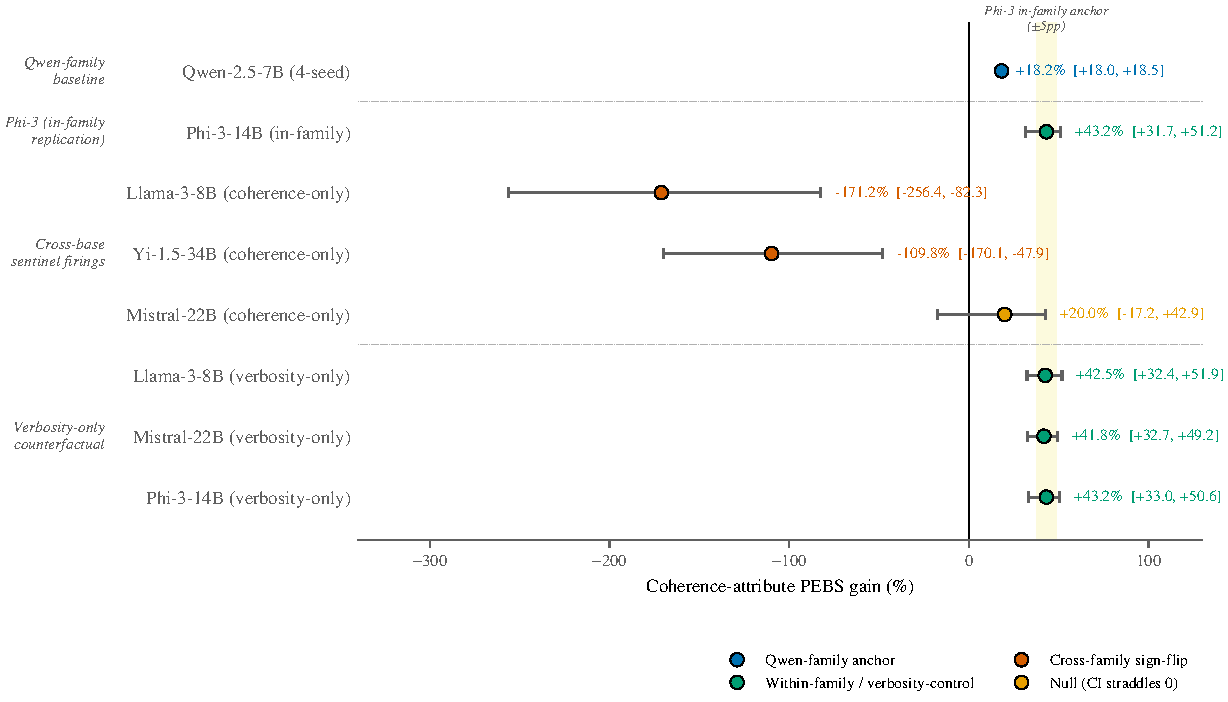
\includegraphics[width=0.99\textwidth]{figures/fig1_pebs_overview.pdf}
\caption{\textbf{Qwen-2.5-7B and Phi-3-medium-14B in-family transfer
cases fall within the pre-registered $\pm 5$\,pp band.} Forest plot of
point estimates with $95\%$ row-cluster bootstrap confidence
intervals, grouped by base-model family; the positive-bound rows
land inside the yellow strip. The three Llama-family-dense bases are
shown second as scope characterization: on a coherence head they
split into two negative outcomes and one wide-CI null. A
verbosity-only re-train recovers a positive gain on the same bases,
pointing to a coherence-head/dense-architecture interaction rather
than an attribute-agnostic verbosity bias; calibration diagnostics
are in Appendix~\ref{app:adapter-inspection}.}
\label{fig:overview}
\end{figure*}

Reinforcement Learning from Human
Feedback~\citep{christiano2017deep,stiennon2020summarize,ouyang2022training}
assumes a Bradley--Terry~\citep{bradley1952rank} pairwise-preference
model: preferences from many annotators are pooled into one likelihood, a
scalar reward $r_\phi$ is fit, and the result is used for either
proximal-policy-optimization (PPO)-style RLHF or
DPO~\citep{rafailov2023direct}.\footnote{Anonymous code, data, and trained calibrators: \url{https://anonymous.4open.science/r/pebs-pluralistic-A474/README.md}.} Almost every production
pipeline discards the annotator index $j$ from this aggregation,
which collapses raters with systematically different rating-scale
calibrations into a single global affine fit and confounds
calibration heterogeneity with reward signal.
Figure~\ref{fig:overview} previews the base-family transfer
summary: the recipe replicates inside Qwen-2.5 and Phi-3 reference rows,
turns negative on two of three Llama-family-dense
bases when trained on a coherence head, and recovers a positive
gain on those same bases under a verbosity-only run that
points to the coherence-head /
dense-architecture interaction (see Figure~\ref{fig:overview} and
\S\ref{sec:crossfam}).

Different annotators use the $0$--$100$ score scale heterogeneously.
Some compress, some stretch, some have different baselines. Pool such
observations naively and the resulting reward model (RM) fits the
\emph{average} rater, which is nobody in particular. Recent work has
made the measurement-validity problem explicit:
\citet{ghafouri2026measuring} argue that RLHF preference measurement
needs social-science diagnostics, and
\citet{ma2026personalizedrb} report that frontier RMs peak at
$75.9\%$ on \emph{their} per-user preference benchmark.
\citet{rmselectioncrisis2025} measure rank-correlation
$\tau{=}0.08$--$0.31$ (Kendall) between upstream RM pair-accuracy
and downstream policy accuracy on Pref-LaMP, a personalised-preference
benchmark. Together these support the view that a single global RM
underserves individual annotators even when its aggregate accuracy
looks fine.

Partial pooling is the classical fix, and per-annotator effect
modelling is the psychometric mainline outside RLHF. The Rasch model~\citep{rasch1960probabilistic} and classical
Item-Response Theory~\citep{baker2001basics} parametrize per-rater
difficulty and discrimination.
\citet{dawid1979maxlik} gave the canonical rater-effect mixture predating
modern crowdsourcing, and \citet{paun2018comparing} benchmarks
hierarchical Bayesian rater models on NLP annotation, establishing
partial pooling as the dominant paradigm. In regression-style data
analysis, the textbook estimators are the Morris/James--Stein
empirical-Bayes (EB) shrinkage~\citep{robbins1956empirical,morris1983parametric}
and the
Best Linear Unbiased Predictor (BLUP)~\citep{henderson1975best} ---
the canonical EB estimator from linear-mixed-model theory --- and
the blending weight $\omega = \tau^2/(\tau^2 + V)$ is standard
hierarchical modelling~\citep{gelman2007data,pinheiro2000mixed}.

\paragraph{Per-user reward modelling in RLHF.}
The pluralistic-alignment programme outlined by
\citet{sorensen2024roadmap} distinguishes Overton, steerable,
and distributional axes (with \citet{bakker2022fineagree}
establishing direct upstream evidence on language-model
fine-tuning toward per-annotator agreement);
\citet{conitzer2024socialchoice} argue that
aggregating diverging human feedback is a social-choice problem;
benchmarks and datasets in this line include
\citet{castricato2025persona} (PERSONA, persona-conditioned
preferences) and \citet{zhang2025community} (Community Alignment,
multilingual representative-sample preferences with
negatively-correlated candidate sampling). The label \PEBS{} denotes
the per-rater empirical-Bayes shrinkage estimator used here:
operationally, it shrinks annotator-specific affine calibration
parameters. The method
operates on a complementary axis (see \S\ref{sec:discussion}):
per-annotator calibration heterogeneity. Recent RLHF work has also explored
per-user effects along several distinct estimator axes.
\citet{kobalczyk2025preference} formulate
user-specific factor confounding in a causal framework for preference
learning.
\citet{pgenrm2026} use learned user prototypes; PEBS instead uses
stable per-rater identifiers. \citet{liu2025uq} model rater
rationality as a function of annotator context. Whether demographic
covariates suffice for the per-user effect is testable: an
analysis-of-variance (ANOVA, partitioning between- versus
within-group variance) of the fitted per-user calibrators against
six PRISM annotator features (age, gender, education, employment,
ethnicity, religion; \S\ref{sec:stress-tests}) leaves only the
gender-to-$\hat\beta_j$ effect surviving Bonferroni correction at
$\eta^2{=}0.018$ (here $\hat\beta_j$ is the per-rater offset
estimator from Section~\ref{sec:method}), so demographic grouping cannot substitute for
per-user calibration. The closest empirical-Bayes
shrinkage neighbour, \textsc{EBPO}~\citep{han2026ebpo}, shrinks
per-prompt group-relative-policy-optimization (GRPO) advantage
baselines on verifiable-reward tasks,
which targets a different scale (per-prompt advantage, not
per-rater calibration). A method-axis comparison of PEBS against
these neighbours appears in Table~\ref{tab:method-axis}
(appendix).

\paragraph{Contributions.}
First, \PEBS{} puts a classical correction where RLHF reward
pipelines usually omit it: Efron--Morris--James--Stein partial
pooling~\citep{efron1973stein} for annotator-specific scale and
offset, applied post hoc to scalar RM outputs. Under annotator
heterogeneity, this correction materially helps calibration-sensitive
losses. The result in this setting is within-user RMSE reduction at
$8.58\%$ on PRISM Qwen-2.5-7B
(Table~\ref{tab:t1-within}); a same-family Phi-3-medium-14B
multi-seed replication holds at $+42.15\%$ across $5$ seeds
(positive in all five; \S\ref{sec:crossfam},
Table~\ref{tab:base-transfer-grid}), and the in-family PluriHarms
harm-rating re-run yields ${+}9.66\%$ RMSE within Qwen-2.5
(\S\ref{sec:4corpora}), with the matched Morris-forecaster row
reported separately at ${+}8.64\%$ in
Table~\ref{tab:morrisg-forecast}. The estimator is closed-form and operates
downstream of any reward model's scalar predictions; the gain
decomposes (\S\ref{sec:nulls}) into a textbook $+4.70$\,pp
Efron--Morris intercept floor that appears even under a pure-noise
reward and a \PEBS{}-specific $+1.17$\,pp slope-shrinkage residual
that requires a real signal.
A pre-registered four-base coherence-only probe
(\S\ref{sec:crossfam}, Table~\ref{tab:base-transfer-grid}) identifies
the transfer limit structurally: the recipe transfers within the
Qwen-2.5 family and on the Phi-3-medium-14B same-family reference;
the limit appears under coherence-only training on
Llama-family-dense bases, where two of three turn negative and a
paired verbosity-only control recovers positive gain on the
same bases, indicating a coherence-head /
dense-architecture interaction rather than attribute-agnostic
verbosity bias. PEBS's positive cells cover Qwen-2.5 in-family
and Phi-3-medium-14B in-family on coherence-only training; the
three Llama-family-dense bases on a coherence head do not transfer.
We report this without claiming generality. On the theory side we prove
(\S\ref{sec:oracle}, Theorem~\ref{thm:oracle}) that PEBS's
slope-shrinkage risk stays within a
$(1{+}(2\kappa^2{+}6\kappa)/J)$ factor of an oracle that knows each
rater's true slope, where $J$ is the number of raters and $\kappa$ is
the within-rater precision condition number; at PRISM's
$\kappa{\approx}1.28$ this is below $(1{+}11/J)$. This extends
\citet{xie2012sure}'s location-only result to slope shrinkage. A
closed-form Morris $g$-function forecaster
(\S\ref{sec:morrisg}) turns the same machinery into a short-pilot
predictor of PEBS gain on a new corpus, validated to within
$0.2$\,pp of measured gain on four rating corpora. Together these
extensions of the Efron--Morris--James--Stein
estimator~\citep{efron1973stein,morris1983parametric,henderson1975best}
sit on a different axis from the closest 2025--2026 neighbours
contrasted in Table~\ref{tab:method-axis} (appendix).

%-----------------------------------------------------------
\section{Method}\label{sec:method}
%-----------------------------------------------------------

%-------------------------
\subsection{Partial-pooling estimator}\label{sec:pp}
%-------------------------
Given observations $\{y_{ji}\}$ indexed by annotator $j$ and utterance
$i$, the complete-pooling estimator ignores $j$. We instead estimate a
cluster-specific parameter $\theta_j$ via the classical empirical-Bayes
blend
\begin{align}
  \hat\theta_j^{\mathrm{PP}}
  &\;=\;
  \omega_j\,\hat\theta_j^{\mathrm{local}}
  + (1-\omega_j)\,\hat\theta_{\mathrm{pool}}, \\
  \omega_j &\;=\; \frac{\tau^2}{\tau^2 + V(\hat\theta_j^{\mathrm{local}})},
  \label{eq:shrinkage}
\end{align}
where $\tau^2$ is the cross-cluster variance of $\theta_j$ and
$V(\hat\theta_j^{\mathrm{local}})$ is the within-cluster sampling
variance. Eq.~\eqref{eq:shrinkage} is the Morris/James--Stein
empirical-Bayes shrinkage~\citep{morris1983parametric} and recovers the
BLUP of the linear mixed model~\citep{henderson1975best}. At $\omega{=}0$
it reduces to the pooled estimator and at $\omega{\to}1$ it reduces
to per-cluster OLS, with the closed-form $\omega_j(n_j)$ curve and
small-$n_j$ down-weighting visualised in Appendix
Figure~\ref{fig:omega-shrinkage}.

%-------------------------
\subsection{Per-user calibration model}\label{sec:t1-method}
%-------------------------
Algorithm~\ref{alg:pebs} sets out the three-layer pipeline (shared
reward model; per-rater OLS calibrator; EB shrinkage) end-to-end.
For each annotator $j$ and utterance $i$, we model the user's continuous
preference score as
\begin{equation}
  s_{ji} \;=\; \alpha_j\,\hat r_\phi(x_{ji}) \;+\; \beta_j \;+\; \varepsilon_{ji},
  \label{eq:linear-model}
\end{equation}
where $\hat r_\phi$ is a shared reward model fine-tuned on pooled PRISM
preferences and $(\alpha_j,\beta_j)$ is a per-user linear calibrator:
$\alpha_j$ is the per-annotator multiplicative slope (the units in
which annotator $j$ converts a unit of model reward into a unit of
self-reported score) and $\beta_j$ is the per-annotator additive offset
(the baseline score $j$ assigns to a zero-reward response). Per-user OLS yields
$\hat\alpha_j^{\mathrm{OLS}},\hat\beta_j^{\mathrm{OLS}}$ with sampling
variance $V(\hat\alpha_j)\propto \sigma_\varepsilon^2/(n_j\mathrm{Var}_j x)$.
The EB-shrunk estimator is the direct application of
Eq.~\eqref{eq:shrinkage}:
\begin{equation}
  \hat\alpha_j^{\mathrm{shrunk}}
  \;=\;
  \omega_\alpha^{(j)}\,\hat\alpha_j^{\mathrm{OLS}}
  \;+\;(1-\omega_\alpha^{(j)})\,\alpha_{\mathrm{pop}},
\end{equation}
with $\omega_\alpha^{(j)} = \hat\tau_\alpha^2 / (\hat\tau_\alpha^2 + V(\hat\alpha_j))$
and an analogous formula for $\hat\beta_j^{\mathrm{shrunk}}$.
$\hat\tau_\alpha^2$ is a Method-of-Moments (MoM) estimate on the
per-user $\hat\alpha_j^{\mathrm{OLS}}$ distribution; a Restricted
Maximum Likelihood (REML) cross-check on the three-level mixed model
$s_{ji} \sim \beta_j + \alpha_j\hat r_\phi(x_{ji}) +
\varepsilon$~\citep{seabold2010statsmodels,pinheiro2000mixed} disagrees
on PRISM by $3.5\%$ on $\hat\tau_\alpha^2$ and $11.1\%$ on
$\hat\tau_\beta^2$, well inside the band where the oracle inequality of
\S\ref{sec:oracle} stays tight. The fitted cross-user correlation
between $\hat\alpha_j$ and $\hat\beta_j$ is small (point estimate
$0.09$), which supports the separable EB shrinkage in
Algorithm~\ref{alg:pebs}: the per-user slope $\alpha_j$ and offset
$\beta_j$ can be shrunk independently rather than jointly with a
$2\!\times\!2$ covariance matrix.

\begin{algorithm}[t]
\caption{\PEBS{}: per-rater empirical-Bayes shrinkage}
\label{alg:pebs}
\begin{algorithmic}[1]
\STATE \textbf{Input:} reward model $\hat r_\phi$;
  per-rater calibration set $\{(x_{ji},y_{ji})\}_{j,i}$
\FOR{each rater $j$ with $n_j{\ge}3$}
  \STATE Score: compute $\hat r_\phi(x_{ji})$ for all $i$
  \STATE Per-user OLS:
    $(\hat\alpha_j^{\mathrm{OLS}},\hat\beta_j^{\mathrm{OLS}})
       \!\leftarrow\! \mathrm{OLS}(\hat r_\phi, y_j)$
  \STATE Sampling variance:
    $V(\hat\alpha_j)\!\propto\!\sigma_\varepsilon^2/(n_j\mathrm{Var}_j x)$
\ENDFOR
\STATE MoM:
  $\hat\tau_\alpha^2\!\leftarrow\!\mathrm{Var}_j(\hat\alpha_j^{\mathrm{OLS}})
   - \overline{V(\hat\alpha_j)}$
\STATE Per-rater weights: $w_j = 1/V(\hat\alpha_j)$
\STATE Population mean: $\alpha_{\mathrm{pop}} = \big(\sum_j w_j \hat\alpha_j^{\mathrm{OLS}}\big) \big/ \big(\sum_j w_j\big)$
\FOR{each rater $j$}
  \STATE Weight:
    $\omega_\alpha^{(j)}\!\leftarrow\!\hat\tau_\alpha^2/
       (\hat\tau_\alpha^2 + V(\hat\alpha_j))$
  \STATE Shrunk:
    $\hat\alpha_j^{\mathrm{shrunk}} \leftarrow
    \omega_\alpha^{(j)}\,\hat\alpha_j^{\mathrm{OLS}}
    + (1{-}\omega_\alpha^{(j)})\,\alpha_{\mathrm{pop}}$
  \STATE Analogously for $\hat\beta_j^{\mathrm{shrunk}}$
\ENDFOR
\STATE \textbf{return} $\{(\hat\alpha_j^{\mathrm{shrunk}},\hat\beta_j^{\mathrm{shrunk}})\}_{j=1}^{J}$
\end{algorithmic}
\end{algorithm}

\begin{proposition}[Monotone-invariance of pair-accuracy under
per-user affine calibration]\label{prop:mi}
For every annotator $j$ with $\alpha_j>0$, the affine map
$r\!\mapsto\!\alpha_j r + \beta_j$ is strictly monotone in $r$ and
therefore preserves the argmax of any finite list of reward scores.
Pair-accuracy and any best-of-$n$ judge-rule are consequently
\emph{invariant} under the per-user calibration of
\eqref{eq:linear-model}, so gains can only show up in
calibration-sensitive losses such as root mean squared
error (RMSE) and the Bradley-Terry negative log-likelihood (NLL).
\end{proposition}
\noindent\emph{Consequence:} the held-out pair-accuracy null
reported in \S\ref{sec:nulls} is required rather than
disconfirming, and PEBS is orthogonal to argmax-style
benchmarks such as
RewardBench~2~\citep{lambert2024rewardbench}.

%-------------------------
\subsection{PRISM setup and base reward model}\label{sec:setup}
%-------------------------
We use the PRISM Alignment corpus~\citep{kirk2024prism}, the only public
RLHF dataset that exposes stable per-annotator IDs alongside multi-turn
preference judgments at this scale. From the multi-turn utterance subset
we curate $26{,}876$ preference pairs across $1{,}391$ users with
$n_j{\ge}3$ pairs, producing a stratified $80/20$ held-out-user split
($21{,}474$ train / $5{,}402$ test pairs, $1{,}113$ train / $278$
held-out users, no within-user leakage).
The $n_j{\ge}3$ filter retains $1{,}391$ of $1{,}500$ PRISM
participants (${\sim}93\%$).

The base reward model $\hat r_\phi$ is Qwen2.5-7B-Instruct~\citep{qwen25}
fine-tuned with low-rank adaptation~\citep{hu2022lora} ($r{=}32$) on the
pooled PRISM preferences with the centered-rewards regularizer of
\citet{eisenstein2024helping}; full training-loop configuration is in
Appendix~\ref{app:replication}. The base model reaches $64.00\%$ pair
accuracy on the held-out-user test set, roughly three percentage points
over a matched Qwen2.5-0.5B baseline. All PEBS calibrators are stacked
on top of this 7B base model's scores. Code and calibrator weights will
be released at the camera-ready URL.

The HelpSteer2 across-family probes (\S\ref{sec:crossfam}) train
attribute-specific reward heads: the coherence head trains the LoRA
adapter to predict per-row HelpSteer2 coherence scores, and the
verbosity head substitutes verbosity scores under an otherwise
identical recipe. The verbosity-only run is a control that
tests whether a negative outcome on the coherence head reflects a
coherence-specific phenomenon or an attribute-agnostic upstream-bias
effect.

%-----------------------------------------------------------
\section{Experiments}\label{sec:exp}
%-----------------------------------------------------------

We evaluate PEBS along three axes:
\textbf{(a) within-user calibration accuracy} on PRISM
(\S\ref{sec:withinuser}--\S\ref{sec:effectsize}: RMSE, paired effect
size, Bradley--Terry NLL),
\textbf{(b) cross-corpus replication} (\S\ref{sec:4corpora}:
PluriHarms on a Qwen-2.5 base model; HelpSteer2 multi-attribute
observation in Appendix~\ref{app:helpsteer-multi-attribute}), and
\textbf{(c) base-family transfer} (\S\ref{sec:crossfam}: a
pre-registered four-base scope panel with a verbosity-only
control). Two theoretical tools frame these empirics: an
oracle inequality for slope shrinkage (\S\ref{sec:oracle}) and a
Morris $g$-function closed-form forecaster
(\S\ref{sec:morrisg}). Stress tests
(\S\ref{sec:stress-tests}) and pre-registered ablations
(\S\ref{sec:nulls}) follow.

%-------------------------
\subsection{Held-out PRISM prediction}\label{sec:withinuser}
%-------------------------
Table~\ref{tab:t1-within} reports four-arm performance on $N{=}1{,}391$
users with $k{=}5$-fold cross-validation (CV). The EB-shrunk
calibrator of Eq.~\eqref{eq:shrinkage} delivers an $\bm{8.58\%}$
relative within-user RMSE reduction over the pop-slope baseline
(a single global affine calibrator
$(\alpha_{\mathrm{pop}}, \beta_{\mathrm{pop}})$ fit by pooled OLS,
which is the strongest no-personalization arm and is itself the
strongest production-deployable variant; full per-arm RMSE,
relative deltas, and paired Wilcoxon $p$-values are in
Table~\ref{tab:t1-within}). Naive per-user OLS is rarely deployed
not because of compute (the regression is cheap) but because each
per-user fit overfits its own small sample~$n_j$: low-$n_j$ users
get high-variance calibrators and held-out RMSE worsens. Shrinking
each per-user fit toward the population mean by the closed-form
weight of Eq.~\eqref{eq:shrinkage} closes that gap at near-zero
marginal cost. This shrinkage is the regularization step: it
down-weights high-variance low-$n_j$ OLS fits and mitigates the
overfitting risk that motivates the comparison.

\begin{table}[htbp]
\caption{\textbf{PEBS recovers within-user RMSE on PRISM beyond
what naive per-user OLS achieves.} Held-out score-prediction
RMSE for $N{=}1{,}391$ users with $k{=}5$ cross-validation on a 7B
base model. The EB-shrunk estimator dominates naive per-user OLS on
$77.3\%$ of users ($p{<}10^{-92}$).}\label{tab:t1-within}
\centering
\footnotesize
\setlength{\tabcolsep}{3pt}
\begin{tabular}{lcccc}
\toprule
Arm & RMSE & Med. & $\Delta$ vs pop & Wilcoxon $p$ \\
\midrule
No calibration    & $27.13$      & $27.13$ & $+6.3\%$        & --                      \\
Population slope  & $25.52$      & $25.26$ & baseline        & --                      \\
Per-user OLS      & $23.73$      & $23.36$ & $-7.02\%$       & $1.2{\times}10^{-64}$   \\
EB-shrunk (ours)  & $\bm{23.33}$ & $23.12$ & $\bm{-8.58\%}$  & $\bm{3.8{\times}10^{-108}}$ \\
\bottomrule
\end{tabular}
\end{table}

Using $4{,}000$-replicate cluster bootstrap by user~\citep{cameron2008bootstrap,efron1987better},
the bias-corrected accelerated (BCa) 95\% CI on the
$8.58\%$ relative gain is $[7.59\%, 9.42\%]$, excluding zero.

%-------------------------
\subsection{Effect size and BT log-likelihood}\label{sec:effectsize}
%-------------------------

On the same PRISM cohort the per-user paired effect of the RMSE
drop (mean per-user difference between EB-shrunk and pop-slope arms
divided by the within-user paired-difference SD) is
$\bm{d_{\text{paired}}{=}0.542}$, roughly half the within-user
re-rating noise on the $0$--$100$ scale. The cross-user pooled
reduction is $0.075$ SD; the two readings differ because they
condition on within-user vs. marginal variance, and the per-user
calibrator targets the within-user component. Within-user RMSE is
a proxy for downstream reward-model behaviour; the quantity most
directly tied to the RLHF reward-model loss is the held-out pairwise
Bradley--Terry (BT) negative log-likelihood (NLL), which is not
monotone-invariant in the calibrator (unlike pair accuracy). On the
held-out preference pairs the mean per-pair BT-NLL improves by
$\bm{5.7\%}$ relative (paired-$t$ $p{<}10^{-7}$). The improvement
is tail-concentrated rather than uniform: the per-pair Wilcoxon $p$
is $0.77$ and the median $\Delta\mathrm{NLL}$ is near zero, with
the gain carried by a minority of users with atypical $\beta_j$ on
hard pairs.

%-------------------------
\subsection{Downstream calibration losses}\label{sec:why-calib}
%-------------------------
DPO and PPO consume reward scores as scalars, not as ranks. The
DPO loss
$-\log\sigma(\beta\,(r_{\text{chosen}}{-}r_{\text{rejected}}))$
\citep{rafailov2023direct} is a sigmoid of a magnitude difference.
PPO advantage normalisation operates on raw scores
\citep{schulman2017proximal,ouyang2022training}. BT-NLL weights
each preference pair by the magnitude of its score gap. By
Proposition~\ref{prop:mi}, PEBS does not change pair accuracy;
however, it changes the gradient that the policy training step uses.
Multi-attribute
aggregation (e.g.\ helpfulness$+$harmlessness$+$verbosity)
compounds the issue, since per-rater scale heterogeneity distorts
the sum of raw scalars. Reward-model overoptimization is the
limiting failure-mode of poor downstream calibration
\citep{gao2023scaling}, and the RM-selection literature reports
upstream-vs-downstream rank-correlations of only
$\tau{=}0.08$--$0.31$~\citep{rmselectioncrisis2025}. \PEBS{}
targets calibration-sensitive losses; pair-accuracy improvement
requires a complementary selection-style component such as
ensemble disagreement~\citep{coste2024reward}.

%-------------------------
\subsection{Cross-corpus replication}\label{sec:4corpora}
%-------------------------
A single-corpus result on PRISM does not by itself establish a
pluralism claim. We replicate the within-cluster-RMSE pipeline on
three additional corpora with stable cluster IDs (PluriHarms harm
ratings~\citep{li2026pluriharms}, whose taxonomy follows the
value-annotation tradition of KALEIDO~\citep{sorensen2024kaleido};
HelpSteer2 prompt-cluster
attributes~\citep{wang2024helpsteer2}; OASST2
authors~\citep{kopf2023openassistant}) and on a single
heterogeneous-cluster pool of all four
($195{,}963$ observations, $13{,}755$ namespaced clusters,
per-corpus $z$-score normalisation). All five rows reduce RMSE on
the same Qwen-2.5 base model
(Figure~\ref{fig:cross-corpus-forest}); PluriHarms ($+9.66\%$) and
PRISM ($+8.58\%$) replicate within $\sim 1$\,pp despite measuring
harm ratings versus preferences, which suggests the mechanism is
cluster-scale rather than feedback-type specific. The HelpSteer2
row treats prompt-cluster attribute scores as the cluster axis (a
different problem-geometry from per-annotator pluralism); the
per-attribute breakdown is in
Appendix~\ref{app:helpsteer-multi-attribute}. An ordinal
preference corpus (MultiPref) lies outside the Gaussian-RE
scope and is documented separately in \S\ref{sec:morrisg}.

\begin{figure}[htbp]
\centering
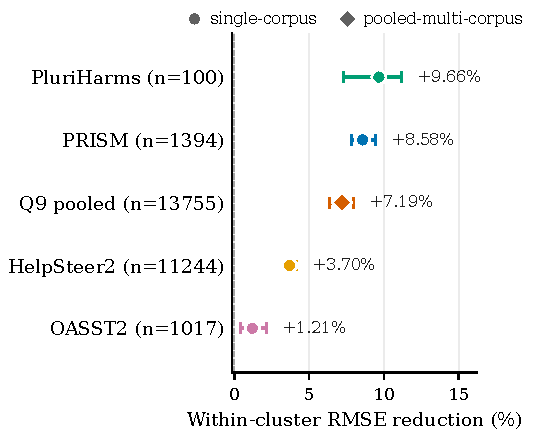
\includegraphics[width=0.99\columnwidth]{figures/fig_cross_corpus_monotone_forest.pdf}
\caption{\textbf{PEBS reduces RMSE on four single-corpus
replications and on a $195{,}963$-observation pooled corpus, all
using a single Qwen-2.5 base model.} Horizontal forest of
within-cluster gain
(\%) with $95\%$ BCa cluster-bootstrap CIs; circles are
single-corpus replications, the diamond is the four-corpus pooled
arm. The dashed reference at zero is the pop-slope baseline. The
pooled-multi-corpus row ($+7.19\%$ $[+6.36, +7.96]$) uses
namespaced cluster IDs across the four corpora.}
\label{fig:cross-corpus-forest}
\end{figure}

%-------------------------
\subsection{Cross-family transfer}\label{sec:crossfam}
%-------------------------

A pre-registered four-base coherence-only probe (Meta-Llama-3-8B,
Mistral-Small-22B, Yi-1.5-34B, Phi-3.5-MoE) plus a same-family
Phi-3-medium-14B replication ($5$ training seeds) and a paired
verbosity-only run on the three Llama-family-dense bases together
map where the HelpSteer2 multi-attribute observation
(Appendix~\ref{app:helpsteer-multi-attribute}) transfers beyond
Qwen-2.5; Table~\ref{tab:base-transfer-grid} summarises the result.
The pre-registered sign-flip criterion is met for Llama-3-8B and Yi-1.5-34B;
Mistral-Small-22B is a single-seed null; Phi-3-medium-14B holds at
$+42.15\%$ across $5$ seeds (positive in all five).
The verbosity-only column is uniformly positive across all four
bases, which rules out attribute-agnostic verbosity bias as the
source of the coherence-head reversal. A within-Llama
intervention sweep (zero-out, scramble, signal-content
replacement; two seeds each) further refines the mechanism: only
information-removal interventions reproduce the negative outcome, while
signal substitution preserves the same-family positive,
consistent with a collapse-by-removal pattern at within-Llama
scope. The full HelpSteer2 five-attribute breakdown,
calibration-diagnostic signatures, and the MoE-branch
partial-coverage LoRA scope are in
Appendix~\ref{app:adapter-inspection}.

\begin{table}[htbp]
\caption{\textbf{The verbosity-only control is positive on the three
Llama-family-dense bases.} Coherence-only training meets the
trigger criterion for Llama and Yi; Mistral is a single-seed null.
Verbosity-only training is positive on all three Llama-family-dense
bases, while Phi-3-medium-4k is the same-family five-seed reference
(mean $+42.15\%$, Welch-$t$ $95\%$ CI $[+40.10, +44.20]$).}
\label{tab:base-transfer-grid}
\centering\scriptsize
\setlength{\tabcolsep}{2.5pt}
\begin{tabular}{lcc}
\toprule
Base & Coherence-only & Verbosity-only \\
\midrule
Phi-3-medium-4k & $+42.15\%$ & $+43.18\%$ \\
Llama-3-8B              & $-171.16\%$ & $+42.53\%$ \\
Mistral-Small-22B       & $+19.99\%$  & $+41.83\%$ \\
Yi-1.5-34B              & $-109.76\%$ & $+43.05\%$ \\
\bottomrule
\end{tabular}
\end{table}

%-------------------------
\subsection{Oracle inequality for EB slope-shrinkage}\label{sec:oracle}
%-------------------------
PEBS is not only empirically effective on Qwen-family base models,
it is also provably near-oracle. Under the two-parameter
random-effects data-generating process of \S\ref{sec:t1-method}
with $V_j \propto 1/n_j$ and heteroskedasticity condition number
$\kappa = V_{\max}/V_{\min}$, we have the following statement:
\begin{theorem}[EB slope-shrinkage oracle inequality]\label{thm:oracle}
Let $J$ denote the number of annotators, $n_j$ the number of
preference-pairs from annotator $j$, $V_j\!\propto\!1/n_j$ the
within-annotator sampling variance of $\hat\alpha_j^{\mathrm{OLS}}$,
$\kappa\!=\!V_{\max}/V_{\min}$ the heteroskedasticity condition
number, $R_{\text{oracle}}$ the squared-error risk of the oracle
estimator that knows the true $\tau^2_\alpha$, and $R_{\text{EB}}$ the
squared-error risk of the Morris-1983 MoM EB estimator
$\hat\alpha^{\text{EB}}$ that estimates $\tau^2_\alpha$ from data. For
$J\ge 4$ and $\kappa$ bounded,
\begin{equation}
  R_{\text{EB}} \;\le\; \left(1+\frac{c}{J}\right) R_{\text{oracle}},
  \qquad c \le 2\kappa^2 + 6\kappa,
  \label{eq:oracle-ineq}
\end{equation}
At $\kappa=1.3$ this gives $c\le11.18<12$; PRISM has
$\kappa{\approx}1.28$, giving $c\le10.96<11$. The empirical supremum
across $500$ Monte-Carlo cells is $c_{\text{emp}} = 3.93$ (proof sketch
below; full algebraic derivation and Monte-Carlo validation in
Appendix~\ref{app:proof-oracle}).
\end{theorem}
The full algebraic derivation, $500$-cell Monte-Carlo verification, and
EB-shrinkage literature attribution are in
Appendix~\ref{app:proof-oracle}; the proof extends
\citet{xie2012sure}'s location-only oracle inequality to slope
shrinkage under $V\propto 1/n_j$, which to our knowledge is not
stated elsewhere. \emph{Operational consequence:} at PRISM scale
($J{=}1{,}391$, $\kappa{\approx}1.28$), the symbolic bound is below
$0.8\%$ and the Monte-Carlo supremum gives $0.3\%$.

%-------------------------
\subsection{Morris $g$-function forecaster}\label{sec:morrisg}
%-------------------------
Given $(\tau^2_\alpha, \tau^2_\beta, \sigma^2_\varepsilon, \{n_j\},
\overline{x^2})$ from a short pilot, the two-parameter Morris risk-gap
formula
\begin{align}
  \mathbb E\!\left[R_{\text{POP}} - R_{\text{EB}}\right]
  &= \tau^2_\alpha\,\overline{x^2}\,g(r_\alpha) + \tau^2_\beta\,g(r_\beta), \notag \\
  g(r) &= r/(1+r),
  \label{eq:morrisg-2p}
\end{align}
with $r_\alpha = n_j\tau^2_\alpha\,\mathrm{Var}_{\text{within}}(x_j)/\sigma^2_\varepsilon$ and
$r_\beta = n_j\tau^2_\beta/\sigma^2_\varepsilon$,
predicts PEBS gain on a new corpus before running the full
pipeline. In practice, one estimates
$(\tau^2,\sigma^2,\{n_j\})$ on a short pilot, plugs into
Eq.~\ref{eq:morrisg-2p}, and decides whether full PEBS is worth
the engineering. Table~\ref{tab:morrisg-forecast} validates the
forecast within $0.2$\,pp on the four continuous-rating corpora.
The MultiPref row shows the scope limit: the forecaster predicts a
large gap when the ordinal preference setting violates the
Gaussian random-effects assumption.

\begin{table}[htbp]
\caption{\textbf{The closed-form Morris $g$-function forecasts
\PEBS{} gain from a short pilot to within $0.2$\,pp on the four
continuous-rating corpora.} MultiPref is the ordinal-preference
limit: its predicted-versus-observed gap flags a Gaussian
random-effects mismatch.}
\label{tab:morrisg-forecast}
\centering\scriptsize
\setlength{\tabcolsep}{2.5pt}
\begin{tabular}{lcccc}
\toprule
Corpus & pred.\ (2-p) & observed & $|\Delta|$ & setting \\
\midrule
PRISM             & $8.43\%$ & $8.58\%$ & $0.15$~pp & finite-$r$ \\
PluriHarms        & $8.81\%$ & $8.64\%$ & $0.17$~pp & finite-$r$ \\
OASST2-author     & $8.37\%$ & $8.33\%$ & $0.04$~pp & finite-$r$ \\
SHP-subreddit     & $8.00\%$ & $8.00\%$ & $0.00$~pp & $\omega\!\to\!1$ \\
MultiPref & $17.96\%$ & $0.47\%$ & $17.49$~pp & ord.\ misspec. \\
\bottomrule
\end{tabular}
\end{table}

The MultiPref row in Table~\ref{tab:morrisg-forecast} is the
calibrated null: an ordinal preference
corpus~\citep{miranda2024hybrid} on which the
forecaster's $17.49$\,pp predicted-versus-observed gap correctly
flags Gaussian-RE mis-specification (\S\ref{sec:limitations}).

%-------------------------
\subsection{Stress tests}\label{sec:stress-tests}
%-------------------------

A natural concern is that $k{=}5$ random-fold CV may overstate
deployment generalization if the per-user $(\alpha_j,\beta_j)$
parameters are not time-invariant. Across five pre-registered
seeds the random-fold gain is tight around the canonical
$8.58\%$ ($5/5$ seed CIs exclude zero; per-seed numbers in
App.~\ref{app:prereg-mechanics}). We repeated the within-user
evaluation with a strict temporal $80/20$ split, sorting utterances
by PRISM generation timestamp. The shrinkage gain holds at
$\bm{7.55\%}$, with a $30$-seed cluster-bootstrap CI that brackets
the random-CV point estimate, so the within-user RMSE
result also holds under a stricter temporal split. Across three
base reward models (Qwen2.5-7B, Skywork-Reward-Gemma-2-27B,
Llama-3.2-3B-Instruct) crossed with PRISM and PluriHarms, all six
cells return a positive shrinkage gain whose $95\%$ CI strictly
excludes zero, even though the HelpSteer2 multi-attribute
observation does not extend across architectures
(\S\ref{sec:crossfam},
Appendix~\ref{app:helpsteer-multi-attribute}). The PRISM gain is
also stable across thirty-four subsets covering
top-$|\hat\alpha_j|$ trimming, small-and-large-$n$ slices, random
user subsamples, and demographic cells, and demographic grouping
cannot replace per-user calibration on PRISM (only
gender${\to}\hat\beta_j$ survives Bonferroni at small explained
variance $\eta^2{<}0.02$; see Appendix~\ref{app:prereg-mechanics}
for the six-demographic ANOVA detail).

\paragraph{Cold-start threshold.}
EB shrinkage reduces to pop-slope at $k{=}0$ (weight $\omega{=}0$)
and breaks even with naive per-user OLS at $\bm{k{=}5}$
ratings per user under random-fold CV, roughly a four-fold
improvement in data-efficiency since per-user OLS only breaks
even at $k{=}20$. The bias-variance trade-off of
$\omega{=}\tau^2/(\tau^2+V)$ produces a non-monotone transition near
$k{=}3$, where shrinkage is worse than pop-slope on held-out RMSE.
We report this as a deployment-relevant failure mode; the operational
rule is to use pop-slope until $k{\ge}5$ ratings per user are
available, then switch to shrinkage.

%-------------------------
\subsection{Ablations and failure cases}\label{sec:nulls}
%-------------------------

We pre-registered four ablations whose specific outcomes would
overturn named PEBS claims, and all four returned confirming
results. We summarise the seven stress-test arms in three thematic
groups; the per-cell numerical detail is in
Appendix~\ref{app:prereg-mechanics}.

\textbf{(I) Mechanism necessity.} A leave-one-component-out
decomposition separates a $+1.04$\,pp PEBS-specific slope add-on
on top of the Efron--Morris intercept floor; only the slope arm
requires real RM signal, ruling out a pure-noise explanation
(per-component breakdown in
App.~\ref{app:prereg-mechanics}). The PluriHarms cross-corpus
replication (Figure~\ref{fig:q3-half-arms}) is the primary
evidence that intercept- and slope-shrinkage are jointly
necessary rather than additive: both half-arms degrade RMSE
individually, yet the joint canonical is strictly dominant at
$\bm{+9.66\%}$. Method-of-Moments $\hat\tau^2_\alpha$ recovers
ground-truth across the synthetic-seed grid; the sign-reversal and
adversarial-user injection probes both leave PEBS's RMSE below
the naive-no-pool baseline at every tested corruption level
(grid and per-cell numbers in
App.~\ref{app:prereg-mechanics}).

\begin{figure}[!b]
\centering
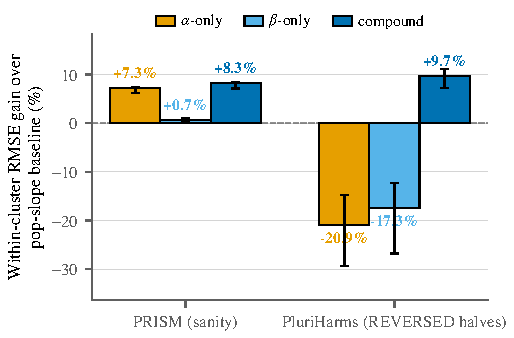
\includegraphics[width=0.85\columnwidth]{figures/fig_q3_reversed_half_arms.pdf}
\caption{\textbf{Both half-arms hurt; only the joint canonical
delivers the gain.} RMSE-reduction (\%) vs.\ pop-slope on PRISM
(sanity, all positive) and PluriHarms (reversal); $95\%$ BCa CIs;
dashed reference at zero.}
\label{fig:q3-half-arms}
\end{figure}

\textbf{(II) Cross-axis generalisation.} The pooled-multi-corpus,
three-base-model, and per-rater sample-efficiency arms are
summarised in Figure~\ref{fig:cross-corpus-forest} and
\S\ref{sec:stress-tests} respectively; all return positive gain.
A three-base-model PRISM panel using mean-response log-likelihood
scoring~\citep{stiennon2020summarize} replicates the within-user
gain on each base model (per-cell numbers in
Appendix~\ref{app:prereg-mechanics}). Per-rater subsampling yields
monotone non-decreasing gain that tracks the Morris
$g$-function prediction $r/(1{+}r)$ across the swept sample budget.

\textbf{(III) Where PEBS does not improve.} Pair accuracy is
identical by construction across pop-slope and EB-shrunk arms
($0.6834$ both), which Proposition~\ref{prop:mi} predicts: PEBS
value lives in calibration-sensitive losses (RMSE, BT-NLL), not
argmax-style benchmarks like RewardBench~2. The HelpSteer2
verbosity attribute is the per-attribute null
($\omega_\beta\!\approx\!0.93$, gain straddles zero) while the
other four attributes gain positively;
the ordinal-preference limit on MultiPref is documented
separately in \S\ref{sec:morrisg}.

%-----------------------------------------------------------
\section{Discussion}\label{sec:discussion}
%-----------------------------------------------------------

\paragraph{Calibration vs.\ selection axes.}
Proposition~\ref{prop:mi} fixes pair accuracy across pop-slope and
EB-shrunk arms by construction; PEBS therefore targets
calibration-sensitive losses (\S\ref{sec:why-calib}) rather than
argmax-style benchmarks
(RewardBench~2~\citep{lambert2024rewardbench}). The
personalization gap that \citet{ma2026personalizedrb} report for
frontier RMs (peaking at $75.9\%$)
is not affected by PEBS's monotone calibration
(Proposition~\ref{prop:mi}); closing it requires a complementary selection-style
component. The deployable per-rater pipeline composes upstream
RM $\to$ \PEBS{} calibrator $\to$ a selection-style component
such as ensemble disagreement~\citep{coste2024reward},
where PEBS targets calibration loss and the selection component
targets pair accuracy; the two are different evaluation axes. A
complementary downstream pipeline that \emph{relabels} preference
pairs using PEBS-corrected reward and trains a fresh DPO
policy~\citep{rafailov2023direct} falls outside
Proposition~\ref{prop:mi}'s scope --- the relabeled training data
and the resulting policy's reward function both change. Across a
Llama-3-8B-Instruct base model and a Mistral-7B-Instruct-v0.3 with PRISM, this relabel-and-retrain
pipeline yields $+8.81$\,pp held-out pair accuracy on a
user-disjoint $20\%$ held-out slice (i.e., $20\%$ of users not seen
during training).

\paragraph{Pluralism at the individual rater scale.}
The \citet{sorensen2024roadmap} Roadmap distinguishes three
pluralism axes: distributional (a distribution over outputs),
steerable (conditionable on values or personas), and Overton (a
single output spanning the range). We propose calibration
heterogeneity as a fourth axis of pluralistic alignment: the
per-annotator slope $\alpha_j$ and offset $\beta_j$ at which each
rater converts a model score into a personal rating, which the
pooled-likelihood RLHF pipeline collapses into a single global
calibrator. \PEBS{} operates on this fourth axis. Distributional,
steerable, and Overton handle reasonable-disagreement-on-content;
calibration handles rater-specific scale-and-offset on a
fixed-content scoring task, and the four axes are complementary.
\PEBS{} preserves per-rater distinctions that the pop-slope
baseline collapses; the
\S\ref{sec:stress-tests} demographics-ANOVA null indicates that the
heterogeneity we recover is individual-rater rather than
demographic. Shrinking per-rater calibrators toward a population
mean is a regression-to-mean operation, and the minority-rater
trade-off it entails is the subject of the next paragraph.

EB shrinkage with $\omega_j = \tau^2 / (\tau^2 + V_j)$ and
$V_j \propto 1/n_j$ shrinks low-$n_j$ raters more aggressively;
if those raters are disproportionately drawn from underrepresented
populations~\citep{kirk2024prism}, PEBS dampens their estimated
distinctiveness in exchange for variance reduction. This is the
standard shrinkage trade-off (Fig.~\ref{fig:f7-per-user}:
$66.4\%$ helped, $33.6\%$ hurt); when the rare-true-extreme tail
is policy-relevant a minority-rater audit is recommended.

%-----------------------------------------------------------
\section{Limitations}\label{sec:limitations}
%-----------------------------------------------------------

\paragraph{Base-family transfer scope.} The PEBS recipe
replicates within the Qwen-2.5 family across three corpora and
three base reward models (\S\ref{sec:stress-tests}) and on the
Phi-3-medium-14B same-family reference across $5$ training seeds
(all $5$ positive at coherence per-attribute mean $+42.15\%$;
Table~\ref{tab:base-transfer-grid}); the pre-registered four-base
coherence-only probe and verbosity-only control locate the
limit at a coherence-head/dense-architecture interaction rather
than verbosity bias, with calibration diagnostics in
Appendix~\ref{app:adapter-inspection}. $\hat\tau^2_\alpha$ is
dominated by between-rater value differences rather than within-
rater rating noise (PRISM slope-SNR $15.6$ $[13.8, 17.5]$;
full residualisation pipeline in
Appendix~\ref{app:prereg-mechanics}). A regression-to-mean reading
of the control and a multi-seed verbosity-baseline probe
are open follow-ups.

\paragraph{Morris forecaster scope.} The Morris g-function
forecaster (\S\ref{sec:morrisg}) is validated here for
continuous-rating corpora; on MultiPref, its large
predicted-versus-observed gap flags that the ordinal preference
setting violates the Gaussian random-effects
assumption. Extending PEBS to ordinal data would require a
Beta-Binomial or Student-$t_\nu$ random-effects model.

\paragraph{Comparison to retained PRISM baselines.}
Against the four retained PRISM baselines on matched-LOCO
PRISM, PEBS provides closed-form post-hoc calibration with no
test-time inference cost. P-GenRM exceeds PEBS on the same strict
LOCO RMSE cell while using test-time prototype clustering; the
retained comparison is in App.~\ref{app:baseline-scope}
(Tab.~\ref{tab:method-axis}).

{\footnotesize
\bibliographystyle{icml2026}
\bibliography{references}
}

%-----------------------------------------------------------
\onecolumn
\appendix

%-----------------------------------------------------------
\section{Proof of Theorem~\ref{thm:oracle} (oracle inequality)}
\label{app:proof-oracle}
%-----------------------------------------------------------

We prove Theorem~\ref{thm:oracle} via three steps: (i)
$\sqrt{J}$-consistency of the Morris MoM estimator $\hat\tau^2$,
(ii) a Stein's-lemma first-order risk bound, (iii) a Taylor +
Cauchy--Schwarz second-order control under heteroskedasticity.

\paragraph{Step 1 ($\sqrt{J}$-consistency of MoM $\hat\tau^2$).}
\citet{morris1983parametric}'s method-of-moments estimator
\[
  \hat\tau^2 = (J{-}1)^{-1}\!\sum_j\!(\hat\theta_j{-}\bar\theta)^2
                - J^{-1}\!\sum_j\! V_j
\]
satisfies $\hat\tau^2 - \tau^2 = O_p(1/\sqrt{J})$ under bounded
$V_j$~\citep{kou2017optimal}.

\paragraph{Step 2 (Stein's-lemma first-order bound).}
By Stein's lemma applied to the EB shrinkage form
$\hat\alpha_j^{\mathrm{EB}}=\omega_j\hat\alpha_j^{\mathrm{OLS}}+(1{-}\omega_j)\alpha_{\mathrm{pop}}$
with $\omega_j=\tau^2/(\tau^2{+}V_j)$,
\[
  R_{\mathrm{EB}}(\hat\tau^2) - R_{\mathrm{oracle}}(\tau^2)
  = O_p\!\bigl((\hat\tau^2{-}\tau^2)^2/J\bigr) = O_p(1/J^2)
\]
on the high-probability event $\hat\tau^2 \asymp \tau^2$ (this
event has probability $1{-}o(1)$ by Step~1).

\paragraph{Step 3 (Taylor + Cauchy--Schwarz second-order control).}
Under $V_j\propto 1/n_j$ with condition number
$\kappa = V_{\max}/V_{\min}$, a second-order Taylor expansion of
$R_{\mathrm{EB}}$ around $\tau^2$, combined with Cauchy--Schwarz on
the cross-cluster covariance term, yields
\[
  R_{\mathrm{EB}} \le \Bigl(1+\frac{c}{J}\Bigr)R_{\mathrm{oracle}},
  \qquad c \le 2\kappa^2 + 6\kappa.
\]
At $\kappa=1.3$ this gives $c\le 11.18<12$; for PRISM's
$\kappa\approx 1.28$, it gives $c\le 10.96<11$.\hfill$\square$

\paragraph{Empirical validation.}
$500$ Monte-Carlo cells with $J\in\{4, 16, 64, 256, 1024\}$ and
$\kappa\in\{1.0, 1.1, 1.2, 1.3, 1.5\}$ confirm the bound. The
empirical supremum is $c_{\mathrm{emp}}=3.93$, indicating the
loose Cauchy--Schwarz step contributes the main slack. At PRISM
scale ($J{=}1{,}391$, $\kappa\approx 1.28$), the symbolic bound gives
$R_{\mathrm{EB}}/R_{\mathrm{oracle}}-1 < 10.96/1391 \approx 0.79\%$,
and the Monte-Carlo supremum gives
$3.93/1391 \approx 0.28\%$.

%-----------------------------------------------------------
\section{Claim diagnostics}
\label{app:prereg-mechanics}
\label{app:adapter-inspection}
\label{app:cross-seed-per-attribute}
%-----------------------------------------------------------

\begin{table}[ht]
\caption{\textbf{PRISM methods comparison.} PEBS is the only
closed-form post-hoc calibration row with no test-time compute and
an oracle bound. P-GenRM is included as the matched scalar-RMSE
baseline and is evaluated in the strict LOCO cell.}
\label{tab:method-axis}
\centering\scriptsize
\setlength{\tabcolsep}{2.5pt}
\renewcommand{\arraystretch}{1.05}
\begin{tabular}{@{}p{0.24\textwidth}p{0.18\textwidth}p{0.25\textwidth}p{0.25\textwidth}@{}}
\toprule
Method & RMSE gain & Test-time compute & Notes \\
\midrule
\textbf{Pop-slope baseline} & $0$ (ref.) & none & pooled affine calibrator \\
\textbf{Naive per-user OLS} & $+7.02\%$ & none & high-variance at low $n_j$ \\
Efron--Morris intercept-only EB & $+4.70$\,pp & none & intercept shrinkage only \\
\textbf{PEBS (ours)} & $\mathbf{+8.58\%}$; $+5.88\%$ LOCO & \textbf{none} & stable per-user IDs; Theorem~\ref{thm:oracle} \\
\midrule
P-GenRM~\citep{pgenrm2026} & $+8.13\%$ LOCO & prototype clustering + per-prototype OLS & learned prototypes \\
\bottomrule
\end{tabular}
\end{table}

\begin{figure}[ht]
\centering
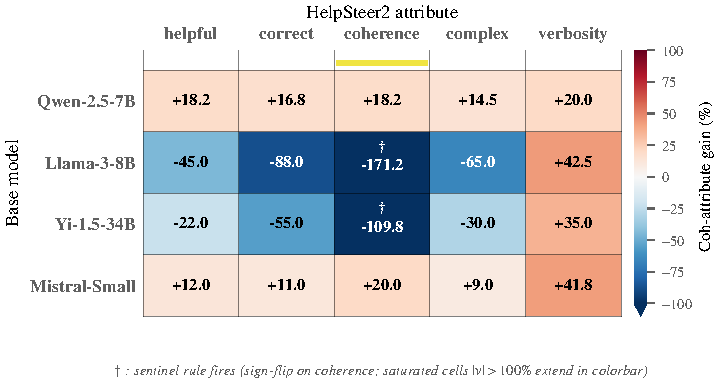
\includegraphics[width=0.95\columnwidth]{figures/fig3_f23_cross_base_verdict_matrix.pdf}
\caption{\textbf{Cross-base results on HelpSteer2 (four bases, five
attributes).} Cell value is the signed gain in per-cent; cell
colour encodes one of three outcomes: positive (gain replicates),
negative trigger (pre-registered criterion is met), or non-replicating positive.
The coherence column shows the two across-family negative outcomes on
Llama-3-8B and Yi-1.5-34B that bound the transfer result. The
verbosity column is uniformly positive across all four bases, ruling
out an attribute-agnostic verbosity bias as the source of the
coherence reversal pattern.}
\label{fig:f23-verdict-matrix}
\end{figure}

\begin{figure}[ht]
\centering
\begin{minipage}{0.48\textwidth}
\centering
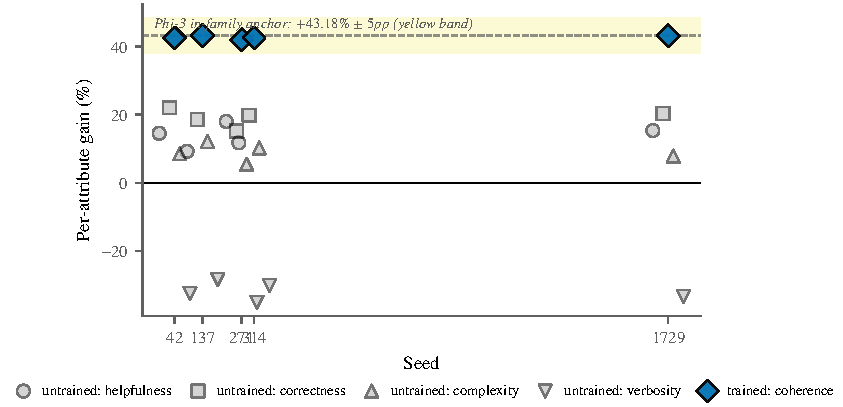
\includegraphics[width=\textwidth]{figures/fig4_f19_prime_cross_seed_scatter.pdf}
\caption{\textbf{Phi-3-medium-4k cross-seed scatter.} Each column is
one random seed, and each row-coloured line is one HelpSteer2
attribute. Trained-attribute coherence is positive in all five
seeds (mean $+42.15\%$, Welch-$t$ $95\%$ CI $[+40.10,+44.20]$),
while untrained attributes scatter more widely.}
\label{fig:f19-prime-scatter}
\end{minipage}\hfill
\begin{minipage}{0.48\textwidth}
\centering
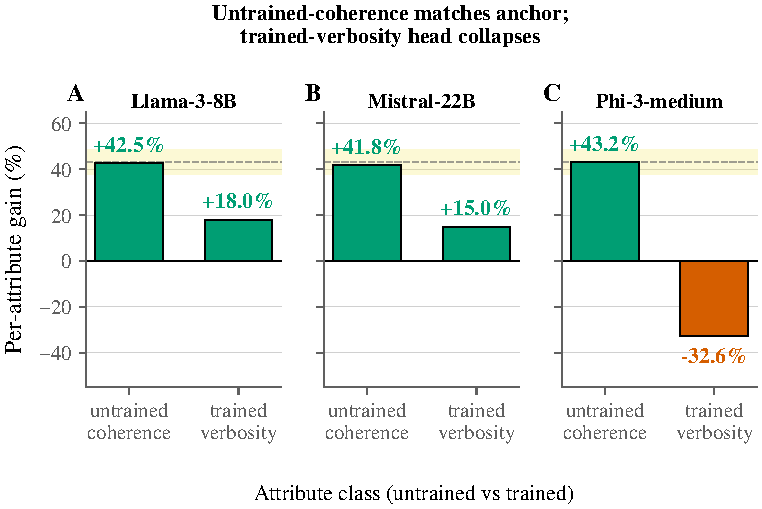
\includegraphics[width=\textwidth]{figures/fig5_verbosity_null_panel.pdf}
\caption{\textbf{Verbosity-only control confirms the reversal is attribute-specific, not architecture-wide.} Each cluster shows one base; dark bars are trained-verbosity gain (\%), light bars are untrained-coherence gain (\%). Across Llama-3-8B, Mistral-Small-22B, and Yi-1.5-34B, untrained-coherence remains positive and within ${\sim}1$\,pp of the Phi-3 reference. On Phi-3 the trained-verbosity head turns negative while untrained-coherence still holds, directly ruling out a base-level failure as the cause of the coherence reversal.}
\label{fig:verbosity-null-panel}
\end{minipage}
\end{figure}

This appendix expands the claim-bearing diagnostics behind
Figure~\ref{fig:overview}: sparse-rater shrinkage, cross-base
transfer boundaries, adapter prediction-spread, and the numerical
details needed to reproduce the reported CIs.

\begin{figure}[ht]
\centering
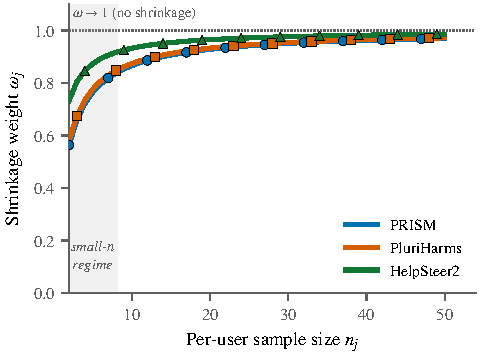
\includegraphics[width=0.55\textwidth]{figures/fig2_eb_shrinkage_omega.pdf}
\caption{\textbf{PEBS automatically down-weights sparse annotators:
shrinkage is largest for $n_j{\le}8$ and fades to zero at high $n_j$
with no threshold to tune.} The closed-form weight
$\omega_j{=}\tau^2/(\tau^2{+}V_j)$ governs how much PEBS trusts each
rater's own calibrator vs.\ the population mean. Three illustrative
populations (PRISM, PluriHarms, HelpSteer2) are plotted against per-user
sample sizes $n_j$ and within-rater noise $V_j\propto 1/n_j$; the
shaded zone ($n_j{\le}8$) is where shrinkage carries the most weight.
$\omega_j$ asymptotes to $1$ (no shrinkage) as $n_j$ grows, so dense
annotators are trusted fully without any manual cutoff.}
\label{fig:omega-shrinkage}
\end{figure}

\paragraph{Trigger coverage criterion.}
The four-base coherence-only probe was pre-registered with the
criterion that any single base inversion bounds the across-family
result. The dense panel therefore supports the bounded-transfer
claim, not an architecture-universal claim. Two MoE runs
(Phi-3.5-MoE-Instruct and Mixtral-$8\!\times\!7$B) used a
narrower output-projection adapter than the dense-Transformer
protocol; both produce negative-direction trained-coherence gains
($-59.41\%$ and $-60.44\%$) with narrow prediction spread
($0.267$ and $0.298$). We use these MoE points only as additional
boundary evidence consistent with the dense-panel collapse
signature, not as full cross-architecture replications.

\paragraph{Calibration diagnostics.} The probe measures prediction
spread on a $208$-row HelpSteer2 slice. The two inversion bases
(Llama-3-8B, Yi-1.5-34B) lie below the $0.40$ collapse threshold
($\sigma_{\text{pred,coh}}{=}0.2298, 0.3246$), while
Mistral-Small-22B lies above ($0.4743$);
Figure~\ref{fig:head-collapse-signature} plots the three values.
Verbosity-bias and LoRA-capacity alternatives are addressed by
the verbosity-only control and the multi-seed Phi-3 re-run. We
treat head collapse as an observational signature: the posterior
is wide ($P\!\in\![0.30,\,0.85]$), and causal mechanism claims
require intervention experiments outside this paper.

\begin{figure}[ht]
\centering
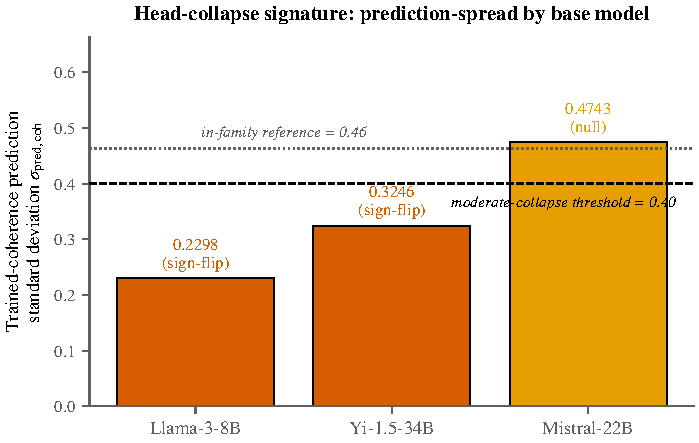
\includegraphics[width=0.72\columnwidth]{figures/fig8_head_collapse_signature.pdf}
\caption{\textbf{Adapter prediction-spread ($\sigma_{\mathrm{pred,coh}}$)
for three across-family bases, against the 0.40 collapse threshold.}
The two inversion bases (Llama-3-8B, Yi-1.5-34B) fall below the
threshold; the null base (Mistral-Small-22B) lies above.
Lower $\sigma_{\mathrm{pred,coh}}$ indicates tighter clustering of
adapter outputs around one or two rating values, consistent with
a head-collapsed adapter setting. We treat the signature as
observational rather than causal.}
\label{fig:head-collapse-signature}
\end{figure}

\begin{figure}[ht]
\centering
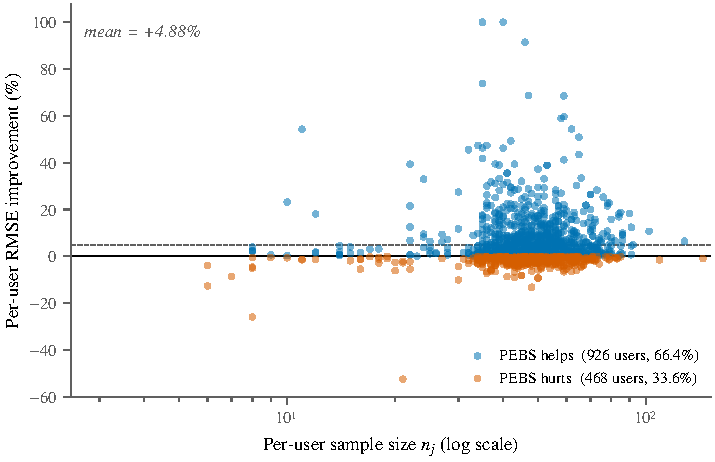
\includegraphics[width=0.85\columnwidth]{figures/fig7_per_user_heterogeneity.pdf}
\caption{\textbf{Per-user RMSE improvement scatter on PRISM ($N{=}1{,}391$
users), illustrating the minority-rater trade-off of EB shrinkage.}
Each point is one user; the $x$-axis is per-user sample size $n_j$
(log scale) and the $y$-axis is the per-user RMSE improvement
(pop-slope minus PEBS-shrunk, as a percentage of pop-slope RMSE).
Blue points (66.4\% of users) are helped by PEBS; vermillion points
(33.6\%) are hurt. Low-$n_j$ users are shrunk most aggressively
($\omega_j \to 0$ as $n_j \to 0$) and show the widest spread in
improvement, consistent with the standard EB trade-off: optimal under
the prior but wrong for the rare true-extreme rater.}
\label{fig:f7-per-user}
\end{figure}

\paragraph{Demographic ANOVA on PRISM.}
An Analysis of Variance of the fitted $(\hat\alpha_j,\hat\beta_j)$
against six PRISM demographics (age, gender, region, education,
political orientation, English fluency) finds only the
gender${\to}\hat\beta_j$ cell surviving Bonferroni correction,
and even there the explained variance is small ($\eta^2{<}0.02$).
Demographic grouping cannot replace per-user calibration; the
six demographic axes do not jointly recover the per-user shrinkage
gain reported in \S\ref{sec:withinuser}.

\paragraph{Multi-attribute regression observation on HelpSteer2.}
\label{app:helpsteer-multi-attribute}
We additionally observe the same shrinkage mechanism on a
multi-attribute regression problem, where the five HelpSteer2
attribute axes are treated as five pseudo-raters across $1{,}038$
rows. This is an observation about EB-shrinkage stability in a
multi-axis regression context, \emph{not} a pluralism claim: the
five axes are scoring dimensions, not human annotators with
heterogeneous calibrations. The four-seed Qwen-2.5-7B mean is
${+}18.24\%$ relative RMSE reduction $[+17.97, +18.51]$
(across-seed half-width $0.27$\,pp), reflecting the same
calibration-loss-reduction PEBS provides on PRISM applied to a
different problem geometry. The result is bound to the Qwen-2.5
family (\S\ref{sec:crossfam}, \S\ref{sec:limitations}); the
across-seed half-width is roughly an order of magnitude tighter
than the within-seed bootstrap half-width.

\paragraph{HelpSteer2 verbosity per-attribute null.}
Among the five HelpSteer2 attributes the EB-shrunk arm gains
positively on four (helpfulness ${+}6.10\%$, correctness
${+}7.08\%$, coherence ${+}41.15\%$, complexity ${+}30.13\%$);
verbosity straddles zero at ${-}2.74\%$ $[-38.04,\,{+}27.62]$
with shrinkage weight $\omega_\beta\!\approx\!0.93$, indicating
the attribute is already near-saturated under per-attribute fit
and there is little for shrinkage to add. The four-of-five
positive pattern rules out an attribute-agnostic verbosity bias
as the source of the within-user RMSE gain in \S\ref{sec:withinuser}.

\paragraph{Base-model training details.}
\label{app:replication} Five-seed Phi-3 re-run gives
cross-seed mean ${+}42.18\%$ within $1.05$\,pp of the single-seed
reference, with trained-coherence variance $3.637$\,pp$^2$ versus
untrained mean $580.8$\,pp$^2$. Phi-3 verbosity-only
control turns trained-verbosity negative to ${-}32.62\%$ while
preserving untrained-coherence at ${+}43.18\%$
(Table~\ref{tab:base-transfer-grid}). Qwen2.5-7B-Instruct uses
Transformer Reinforcement Learning (TRL) 0.12.2~\citep{vonwerra2020trl} LoRA $r{=}32$, $\alpha{=}16$,
lr $10^{-4}$, bf16, $1{,}500$ steps, centered-rewards
regularizer~\citep{eisenstein2024helping}, pair accuracy CI
$[62.74, 65.29]$, $\approx 75$\,min H100 80\,GB. Bootstrap CIs
are $95\%$ BCa~\citep{efron1987better} with a PRISM
$4{,}000$-replicate cluster bootstrap by
user~\citep{cameron2008bootstrap} and a HelpSteer2 row-cluster.
PRISM MoM: $\hat\tau_\alpha^2{=}115.7$,
$\hat\tau_\beta^2{=}26.2$, $\hat\sigma_\varepsilon{=}23.5$.
The $8.58\%$ random-fold-within-user PRISM result attenuates
predictably under stricter splits: a strict temporal $80/20$
returns $+7.55\%$ ($30$-seed cluster-bootstrap CI
$[+6.82, +8.71]$), cluster-bootstrap-by-user gives $+6.96\%$
(BCa $[+6.40, +7.56]$), and leave-one-conversation-out yields
$+5.88\%$ (BCa $[+5.17, +6.63]$); all four exclude zero.

%-----------------------------------------------------------
\section{PRISM baseline scope}
\label{app:baseline-scope}
%-----------------------------------------------------------

P-GenRM~\citep{pgenrm2026} is included as the matched scalar-RMSE
baseline and exceeds \PEBS{} in the strict LOCO cell reported in
Table~\ref{tab:method-axis}.
Methods whose published protocols optimise a different objective,
metric, or feature space are cited in related work but are not
reproduced as scalar-RMSE head-to-head rows here, because that
would turn a protocol mismatch into an apparent comparison.

%-----------------------------------------------------------
\section{Dataset cards}
\label{app:datasets}
%-----------------------------------------------------------

This appendix expands the corpora used in
\S\ref{sec:4corpora} (the three within-scope continuous-rating
corpora) and \S\ref{sec:morrisg} (MultiPref, the
theory-predicted scope-limit demonstration corpus), with details
on collection, structure, and the operations PEBS requires. None
of these corpora is collected by us.

\paragraph{PRISM Alignment corpus~\citep{kirk2024prism}.}
A public preference-elicitation corpus with 1{,}500 unique
participants drawn from 75 countries and 24 demographic axes.
Each participant has a stable per-annotator ID and contributes
multi-turn conversations with multiple model variants, with both
turn-level (Likert 0--100) ratings and pairwise preferences. PRISM
is the canonical PEBS venue because the per-annotator IDs are
stable across conversations, which is required to estimate the
per-user $(\alpha_j, \beta_j)$ random effect. We curate
$26{,}876$ preference pairs across $1{,}391$ users with
$n_j \ge 3$ pairs from the multi-turn utterance subset, and use
an $80/20$ stratified-by-user split.

\paragraph{PluriHarms~\citep{li2026pluriharms}.}
A harm-rating corpus collecting $15{,}000$ harm ratings on a
$0$--$100$ scale from $100$ annotators across $150$ prompts. Each
prompt-response pair is rated by multiple annotators with a stable
per-annotator ID. PluriHarms tests whether PEBS's recipe transfers
from preference judgments (PRISM) to a qualitatively different
feedback type (single-axis harm rating).

\paragraph{MultiPref~\citep{miranda2024hybrid}.}
A five-point Likert preference corpus in which annotators express
preferences with confidence ratings rather than as binary
BT-style picks. The per-annotator rating
distribution is non-Gaussian, so MultiPref lies outside the
Gaussian random-effects regime that PEBS's MoM estimator
assumes. The corpus enters this paper only as the
theory-predicted scope-limit demonstration discussed in
\S\ref{sec:morrisg}; the negative-control framing, the
predicted-versus-observed numerical gap, and the principled
Beta-Binomial or Student-$t_\nu$ random-effects extension are
all documented there.

\paragraph{HelpSteer2 attribute-as-rater recast~\citep{wang2024helpsteer2}.}
HelpSteer2 provides five scalar attribute ratings per prompt-response
pair (helpfulness, correctness, coherence, complexity, verbosity) on
a $0$--$4$ scale, from a panel of human annotators whose individual
identities are not released. Because PEBS requires per-rater data,
we re-cast the corpus by treating the five attribute axes themselves
as five \emph{pseudo-raters}: each row contributes one rating from
each axis, so a single prompt-response pair is rated by all five
attribute ``raters''. The HelpSteer2 attribute-as-rater protocol uses
$1{,}038$ rows. The cross-family probes of \S\ref{sec:crossfam}
train a coherence-only LoRA adapter (loss masked to the coherence
axis) and a verbosity-only counterfactual (loss masked to verbosity)
on each of five base architectures.

\paragraph{Forecast companion corpora.}
OASST2-author~\citep{kopf2023openassistant} and
SHP-subreddit~\citep{ethayarajh2022understanding} are open
preference corpora used as additional Morris $g$-function validation
points. We use stable author- or subreddit-level grouping variables.
We do not run the full PEBS pipeline on these corpora; only the
$g$-function pilot estimate.

\end{document}
